% !TeX spellcheck = de_DE
% !TeX TS-program = pdflatex
\documentclass{beamer}
\usepackage[utf8]{inputenc}
\usepackage[ngerman]{babel}
\usetheme{JuanLesPins}  %% Themenwahl
\usepackage{bytefield}

\usepackage{wasysym}

\usepackage{pgfpages}
\setbeamertemplate{note page}[plain]
\setbeameroption{show notes on second screen=right}

\title{RIOTOIR}
\author{Hauke, Marcel, Martin}
\date{\today}

\begin{document}
	\beamertemplatenavigationsymbolsempty
	\unitlength 5mm

	\maketitle

	\begin{frame} %%Eine Folie
		\frametitle{ RIOTOIR } %%Folientitel
		\begin{block}{\textbf{RIOT} - \textbf{O} - \textbf{IR}}
			\begin{tabbing}
				RIOT \= $\rightarrow$ \= RIOT\\
				\break
				O  	 \> $\rightarrow$ \> On\\
				\break
				IR   \> $\rightarrow$ \> Infrared\\
			\end{tabbing}
		\end{block}
	\end{frame}


	\begin{frame} %%Eine Folie
		\frametitle{ Protokoll } %%Folientitel
		\begin{block}{Header}
			\vspace{0.5cm}
			\begin{center}
				\begin{bytefield}{24}
					\bitheader{0-23}\\
					\bitbox{8}{Version}
					\bitbox{8}{Empfänger}
					\bitbox{8}{Sender}	\\

					\bitbox{8}{Länge}
					\bitbox{8}{Checksumme}
					\bitbox{8}{Nachricht}\\
					\wordbox[tlr]{1}{Nachricht}\\
					\skippedwords\\
					\wordbox[blr]{1}{}
				\end{bytefield}
			\end{center}
			\vspace{0.3cm}
		\end{block}
	\end{frame}

	\note{ Präambel entfernt \\
		Version 0x1 \\
		Adressraum: 255 Stationen}

	\begin{frame} %%Eine Folie
		\frametitle{ Modulation } %%Folientitel
		{\LARGE Idee:}
		\break
		\begin{figure}
			\begin{center}
				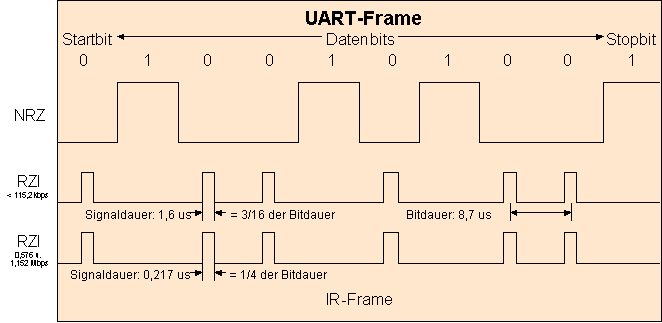
\includegraphics[scale=0.5]{Medien/Modulation.PNG}\\
				Orientiert am Infrared Data Association $IrDA^{\textregistered}$
			\end{center}
		\end{figure}
	\end{frame}

	\begin{frame} %%Eine Folie
		\frametitle{ Modulation } %%Folientitel
		{\LARGE Problem:}\\
		- Timing in RIOT zu niedrig aufgelöst\\
		\break
		{\LARGE Lösung:}\\
		-Weniger Timing\\

	\end{frame}

	\begin{frame} %%Eine Folie
		\frametitle{ Performance } %%Folientitel
		{\Large Max:}\\
		Max Nachrichtennutzlast: $255 Byte - 5 Byte = 250 Byte/Nachricht$\\
		Min Zeit pro Nachricht: $2 * 3,5 ms * 255 Byte/Nachricht = 1785 ms/Nachricht$)\\
		Theoretische max Baudrate: $\frac{1000 ms/s}{\frac{1785 ms/Nachricht}{250 Byte}} = 140 Byte/s$\\
		{\Large Min:}\\
		Min Nachrichtennutzlast: $1 Byte/Nachricht$\\
		Max Zeit pro Nachricht: $2 * 18 ms * 1 Byte/Nachricht = 36 ms/Nachricht$)\\
		Theoretische min Baudrate: $\frac{1000 ms/s}{\frac{36 ms/Nachricht}{1 Byte}} \approx 28 Byte/s$\\

		Theoretische mittlere Baudrate: $\approx 84 Byte/s$

	\end{frame}

	\begin{frame}{Empfänger}
		\begin{itemize}
			\item Interrupts und Message Passing
			\item Dedizierter Thread zum dekodieren
		\end{itemize}
	\end{frame}

	\begin{frame}
		\frametitle{8-Bit CRC Algorithmus} %%Folientitel
		\begin{itemize}
			\item Zur Überprüfung der übertragenen Headerdaten
			\item kein 8-Bit CRC Algorithmus in RIOT vorhanden
			\item auf Polynomdivision basierend
		\end{itemize}
	\end{frame}

	\note{CRC Modul vorhanden\\
		Internet CRC Modul vorhanden\\
		evtl. 8-Bit CRC in RIOT integrieren}

	\begin{frame}
		\frametitle{ Timing }
		\small
		\begin{tabular}{|c|c|c|c|c|}
			\hline
			Datum  & Ereignis & Hauke & Marcel & Martin \\
			\hline
			23.10. & MS2 ready & CRC\checked, Zähler auslesen & Empfangen\checked & Senden\checked \\
			\hline
			29.10. & MS 2 & & &\\
			\hline
			27.11. & MS3 ready & \multicolumn{3}{|c|}{ Itegration Sender/Empfänger \checked} \\
			&  & \multicolumn{3}{|c|}{ Integration in RIOT Netzwerkstack }\\
			&  & \multicolumn{3}{|c|}{ Testumgebung schaffen \checked}\\
			\hline
			03.12. & MS 3 & & & \\
			\hline
			08.01. & Project finish & \multicolumn{3}{|c|}{ Integration der Wettervorhersage } \\
			&  & \multicolumn{3}{|c|}{ Solar-Last-Logik fertig }\\
			&  & \multicolumn{3}{|c|}{ Demo fertig }\\
			\hline
			14.01. & MS 4 & & & \\
			\hline
		\end{tabular}
	\end{frame}


\end{document}
